\documentclass{article}

\usepackage{amsmath}
\usepackage{amssymb}

\usepackage{geometry}

\usepackage{tikz}

\title{Edexcel Advanced Level GCE Mathematics FP2}
\author{William Bevington \and Callum O'Brien \and Alex Pace}
\date{}

\begin{document}

\maketitle
\tableofcontents
\newpage

\section{de Moivre's Theorem}

de Moivre's theorem states:

\[\text{If } z=r\left(\cos\left(\theta\right)+i\sin\left(\theta\right)\right)\]

\[\text{Then } z^n=\left(r\left(\sin\left(\theta\right)+i\sin\left(\theta\right)\right)\right)^n=r^n\left(\cos\left(n\theta\right)+i\sin\left(n\theta\right)\right)\]

\noindent And in the Exponential form:

\[\text{If } z=re^{i\theta}\]

\[\text{Then } z^n=\left(re^{i\theta}\right)^n=r^ne^{i\theta n}\]

\noindent This can be proved through proof by induction by following the following framework:

\begin{itemize}
\item Prove for \(n=1\).
\item Assume true for \(n=k\)
\item Show true for \(n=\left(k+1\right)\)
\item State conclusion.
\end{itemize}

\noindent Prove that: \(\left(r\left(\cos\left(\theta\right)+i\sin\left(\theta\right)\right)\right)^n = r^n\left(\cos\left(n\theta\right)+i\sin\left(n\theta\right)\right)\) \\\\

\noindent When \(n=1\)

\[\text{LHS } = \left(r\left(\cos\left(\theta\right)+i\sin\left(\theta\right)\right)\right)^1=r\left(\cos\left(\theta\right)+i\sin\left(\theta\right)\right)\]

\[\text{RHS } = r^1\left(\cos\left(\left(1\right)\theta\right)+i\sin\left(\left(1\right)\theta\right)\right)=r\left(\cos\left(\theta\right)+i\sin\left(\theta\right)\right)\]

\[\text{RHS } = \text{ LHS}\]

\[\rightarrow \text{True when } n=1\]

\noindent Assume true for \(n=k\)

\[\therefore \hspace{0.2in} \left(r\left(\cos\left(\theta\right)+i\sin\left(\theta\right)\right)\right)^k=r^k\left(\cos\left(k\theta\right)+i\sin\left(k\theta\right)\right)\]

\noindent When \(n=\left(k+1\right)\)

\[\left(r\left(\cos\left(\theta\right)+i\sin\left(\theta\right)\right)\right)^{k+1}=\]

\[=r\left(\cos\left(\theta\right)+i\sin\left(\theta\right)\right)\times r^k\left(\cos\left(k\theta\right)+i\sin\left(k\theta\right)\right) = r^{k+1}\left(\cos\left(\left(k+1\right)\theta\right)+i\sin\left(\left(k+1\right)\theta\right)\right)\]

\noindent Given it is true for \(n=\left(k+1\right)\) when it is true for \(n=k\) ad it is true for \(n=1\), by mathematical induction, it is true for all positive \(n\). \\\\

\noindent The proof for negative integers is a little simpler as because we have proofed it for positive intergers, we can assume it works for them before we even begin!.

\begin{itemize}
\item Let \(n=-m\)
\item Start with left hand side - rewrite as fraction - apply statement.
\item Make the denominator real
\item Simplify \& rearange for the right hand side
\end{itemize}

\noindent \(n=-m\)

\[z^{-m}=\left(r\left(\cos\left(\theta\right)+i\sin\left(\theta\right)\right)\right)^{-m}\]

\[\text{LHS  }=\frac{1}{\left(r\left(\cos\left(\theta\right)+i\sin\left(\theta\right)\right)\right)^m}\]

\noindent We have already proved that de Moivre's theorem works for positive integers so we can simplify tis further without having to explain anything:

\[\text{LHS  }=\frac{1}{r^m\left(\cos\left(m\theta\right)+i\sin\left(m\theta\right)\right)}\]

\noindent Make the denominator real by multiplying by the complex conjugate

\[\text{LHS  }\times\frac{\left(\cos\left(m\theta\right)-i\sin\left(m\theta\right)\right)}{\left(\cos\left(m\theta\right)-i\sin\left(m\theta\right)\right)}=\frac{\left(\cos\left(m\theta\right)-i\sin\left(m\theta\right)\right)}{r^m\left(\cos^2\left(m\theta\right)+\sin^2\left(m\theta\right)\right)}\]

\noindent Trigonometric identities tell us that:

\[\cos^2\left(m\theta\right)+\sin^2\left(m\theta\right)=1\]

\noindent and

\[\cos\left(m\theta\right)=\cos\left(-m\theta\right)\]
\[-\sin\left(m\theta\right)=\sin\left(-m\theta\right)\]

\noindent Applying these to the LHS results in a fraction that is easily manipulated to our RHS:

\[\text{LHS  }=\frac{\left(\cos\left(-m\theta\right)+i\sin\left(-m\theta\right)\right)}{r^m}\]

\[\text{LHS  }=r^{-m}\left(\cos\left(-m\theta\right)+i\sin\left(-m\theta\right)\right)=\text{  RHS}\]

\noindent de Moivre's Theorem is very useful, as it can be applied to simplify complicated looking expressions: \\\\

\noindent \textit{Simplify:}

\[\frac{\left(\cos\left(\frac{9\pi}{17}\right)+i\sin\left(\frac{9\pi}{17}\right)\right)^5}{\left(\cos\left(\frac{2\pi}{17}\right)-i\sin\left(\frac{2\pi}{17}\right)\right)^3}\]

\noindent First we must put the denominator into the correct polar form (with a \(+\) inbetween cos and sin), and then we can apply de Moivre's Theorem.

\[\frac{\left(\cos\left(\frac{9\pi}{17}\right)+i\sin\left(\frac{9\pi}{17}\right)\right)^5}{\left(\cos\left(\frac{-2\pi}{17}\right)+i\sin\left(\frac{-2\pi}{17}\right)\right)^3}\]

\noindent And now appying de Moivre's Theorem:

\[\frac{\cos\left(\frac{45\pi}{17}\right)+i\sin\left(\frac{45\pi}{17}\right)}{\cos\left(\frac{-6\pi}{17}\right)+i\sin\left(\frac{-6\pi}{17}\right)}\]

\noindent From this point we can easily simplify the complex number down.

\[\cos\left(\frac{51\pi}{17}\right)+i\sin\left(\frac{51\pi}{17}\right)\]

\[\cos\left(3\pi\right)+i\sin\left(3\pi\right)\]

\[\cos\left(\pi\right)+i\sin\left(\pi\right)=-1\]

\subsubsection{de Moivre's Theorem and Trigonometric Identities}

de Moivre's Theorem can also be applied to problems consisting of trigonometric functions by using identites and binomial expansion. First though, it is worth noting the following, where \(Z\) is a complex number \(r\left(\cos\left(\theta\right)+i\sin\left(\theta\right)\right)\)

\[\begin{array}{cc} 
            \vspace{15pt} Z+\frac{1}{Z} \:=\: 2\cos\left(\theta\right) \hspace{10pt} & Z^n+\frac{1}{Z^n} \:=\: 2\cos\left(n\theta\right) \\
            Z-\frac{1}{Z} \:=\: 2i\sin\left(\theta\right) \hspace{10pt} &  Z^n-\frac{1}{Z^n} \:=\: 2i\sin\left(\theta\right)
\end{array}\]

\noindent Trigonometric functions can be replaced with these arrangements of complex numbers and then manipulated far more easily. The following is an example of such a situation. \\

\noindent Express \(\sin^3\left(\theta\right)\) in the form \(d\cos\left(4\theta\right)+e\cos\left(2\theta\right)+f\)

\[Z-\frac{1}{Z} \:=\: 2i\sin\left(\theta\right) \;\therefore\; \left(Z^4-\frac{1}{Z^4}\right)^4 \:=\: 16\sin\left(4\theta\right)\]
\[\left(Z^4-\frac{1}{Z^4}\right)^4 \:=\: Z^4+4Z^3\left(\frac{-1}{Z}\right)+6Z^2\left(\frac{-1}{Z}\right)^2+4Z\left(\frac{-1}{Z}\right)^3+\left(\frac{-1}{Z}\right)^4\]
\[\rightarrow\: Z^4+4Z^2+6-4Z^{-2}+Z^{-4}\]
\[\rightarrow\: \left(Z^4+\frac{1}{Z^4}\right)-4\left(Z^2+\frac{1}{Z^2}\right)+6\]
\[\therefore\: 16\sin^4\left(\theta\right) \:=\: 2\cos\left(4\theta\right)-8\cos\left(2\theta\right)+6\]
\[\therefore\: \sin^4\left(\theta\right) \:=\: \frac{1}{8}\cos\left(4\theta\right)-\frac{1}{2}\cos\left(2\theta\right)+\frac{3}{8}\]

\subsubsection{Finding the nth Root of a polynomial Using de Moivre's Theorem}

Solve \(Z^3=1\). Represent Solutions on an argand diagram.

\[|Z^3|=1 \;\; arg(Z^3)=\pi\]
\[Z^3=1\left(\cos\left(\pi\right)+i\sin\left(\pi\right)\right)\]
\[Z^3=\left(\cos\left(\pi+2k\pi\right)+i\sin\left(\pi+2k\pi\right)\right)\]
\[Z=\left(\cos\left(\pi+2k\pi\right)+i\sin\left(\pi+2k\pi\right)\right)^{\frac{1}{3}}\]
\[Z=\cos\left(\frac{\pi+2k\pi}{3}\right)+i\sin\left(\frac{\pi+2k\pi}{3}\right)\]

\noindent We only need consider all values of k for which \(\pi<\theta<\pi\)

\[k=0 \;\rightarrow\; Z=\cos\left(\frac{\pi}{3}\right)+i\sin\left(\frac{\pi}{3}\right)\]
\[\therefore \; Z \:=\: \frac{1}{2}+\frac{\sqrt{3}}{2}i\]
\[k=1 \;\rightarrow\; Z=\cos\left(\pi\right)+i\sin\left(\pi\right)\]
\[\therefore \; Z \:=\: -1\]
\[k=-1 \;\rightarrow\; Z=\cos\left(\frac{-\pi}{3}\right)+i\sin\left(\frac{-\pi}{3}\right)\]
\[\therefore \; Z \:=\: \frac{1}{2}-\frac{\sqrt{3}}{2}i\]

\begin{center}
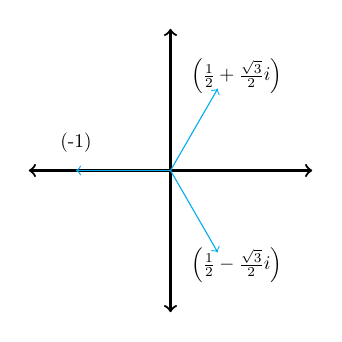
\begin{tikzpicture}[xscale=1.2,yscale=1.2]
    \draw[thick, <->] (-1.5,0) -- (1.5,0);
    \draw[thick, <->] (0,1.5) --(0,-1.5);
    \draw[cyan, ->] (0,0) -- (-1,0);
    \draw[cyan, ->] (0,0) -- (0.5,0.866);
    \draw[cyan, ->] (0,0) -- (0.5,-0.866);
    \node[scale=0.7] at (-1,0.3) {(-1)};
    \node[scale=0.7] at (0.7,1) {\(\left(\frac{1}{2}+\frac{\sqrt{3}}{2}i\right)\)};
    \node[scale=0.7] at (0.7,-1) {\(\left(\frac{1}{2}-\frac{\sqrt{3}}{2}i\right)\)};
\end{tikzpicture}
\end{center}


\end{document}
